\chapter{State of the Art}
\label{chap:stateoftheart}
TODO: outline if the chapter


\section{Electromagnetic Exposure}

\subsection{Electromagnetic Field Radiation} % (fold)
\label{sub:emf}
People in a telecommunication network are exposed to far field electromagnetic radiation originating from base stations and other \gls{UE}. 
Network planners need to make sure that the electromagnetic fields (expressed in V/m) do not exceed limitations enforced 
by the government. These limits are location dependent. The European Union recommends the guidelines as defined by the \gls{ICNIRP} which limits electromagnetic exposure to 61 V/m.
Each European country needs to decide for themselves which limitations to enforce. Belgium for example delegated this responsibility to Flanders, Brussels and Wallonia \cite{J23}.

The used deployment tool is applied in Ghent, a Flemish city in Belgium. The standards defined by the Flemish government are therefore applicable.
They state that in the 2.6 GHz frequency band, an individual antenna cannot exceed 4.5 V/m and the cumulative sum of all fixed sources has its maximum at 31 V/m \cite{J23, S13_normenBelgie}.

\subsection{Specific Absorption Rate}
\gls{SAR} represents the rate at which electromagnetic energy is absorbed by human tissue with the thermal effect as its most important health consequence.
The volume of this tissue is typically 1 g or 10 g. The \gls{FCC} of the \gls{USA} defines regulations based on 1 g tissue (indicated as $SAR_{1g}$) 
while the European Union handles the 
10 g model ($SAR_{10g}$). $SAR$ values can further be categorized based on the area it covers, as an example, 
the whole body \gls{SAR} ($SAR^{wb}$)is defined as the average radiation over the entire body.
Another  example are localized \gls{SAR}-values that only cover a certain part of the human body like the head.
The \gls{ICNIRP} has concluded that the threshold effect for $SAR^{wb}_{10g}$ is at 4 W/kg meaning that any higher absorption rate would overwhelm the \gls{thermoregulatory capacity} of the human body.
Whole body values between 1 and 4 W/kg increase the temperature of human body less than 1°C, which is proven not to be harmful for a healthy human being\cite{J24}.
Thereafter, a safety margin is introduced to tackle unknown variables like experimental errors, increased sensitivity for certain population groups and so on. 
This results in a whole body $SAR_{10g}$ of $0.8 W/kg$ and $2 W/kg$ for localized $SAR_{10g}$ at head and torso area \cite{J23, S13_normenBelgie}.
An overview is given in table \ref{table:overviewSARValues}

%todo: de 10g slaat al op localized, vandaar dat het maar 10g is, anders is het whole-body
%todo: we kunnen niet sar10gmax gebruiken want This means that the SAR calculations will be worst-case and possibly an overestimation of the real localised SAR. (herwoorden voor plagiaat)
%Human exposure caused by downlink traffic is a not negligible asset. However, telecommunications is not a one-way street. When connecting to a UMTS network, also uplink data caused by the \gls{UE} should be considered.
%\gls{UE} generates, just like femtocells, electromagnetic waves to which a user is exposed. A part of this radiation goes to the femtocell, another part enters the body of its user. How much electormagnic strenghts enters the body is defined as \gls{SAR} and is measured with 10g biological tissue which represents the human skin. This value will from now on be expressed as $SAR_{10g}$. 
%A mobile device induces two types of exposure: local and whole-body. 

\begin{table}[]
\begin{tabular}{|l|c|}
\hline
\textbf{Description} & \textbf{Value} \\ \hline
Maximum $SAR^{wb}_{10g}$ as defined by \gls{ICNIRP}                           &  $4 W/kg$              \\ \hline
Maximum $SAR^{wb}_{10g}$ as defined by the Belgian government                  & $0.8 W/kg$               \\ \hline
Maximum $SAR_{10g}$ for head and torso as defined by the Belgian government                  & $2 W/kg$               \\ \hline
\end{tabular}
\label{table:overviewSARValues}
\caption{Overview of the different \gls{SAR} limitations.}
\end{table}
TODO:  is dit voor heel belgie of voor vlaanderen?


\subsection{Related Work} % (fold)
\label{sub:general}
The goal of this master dissertation is the investigation of electromagnetic exposure considering all sources. Three types of sources are considered: electromagnetic radiation 
caused by base stations, near field radiation from the user's own device and far field radiation originating from other users' equipment. This electromagnetic radiation is thereafter
absorbed by the human body which will be expressed in SAR values.

Several papers calculate exposure originating from certain sources, but very  limited research has been done covering the whole picture.
In \cite{J6_originalExposureFormula} is described how electromagnetic radiation of several WiFi access points is being calculated. The authors of \cite{J1} used this knowledge 
to investigate electromagnetic exposure originating from base stations in a more outdoor environment. \cite{J10_RDP, J10.1} addresses the fact that 
also \gls{UL} traffic from the user's device should be considered. They therefore investigated indoor exposure. They did not only consider the electromagnetic radiation
but also how much is absorbed by the body, which will be expressed as specific absorption rate. Since the authors only covered voice calls,
uplink SAR was expressed in localized SAR values while the downlink traffic is expressed in whole body SAR. With the advent of 5G, paper \cite{J17_kuehn2019modelling} has been 
published, describing how localized SAR values are achieved from all sources. More precisely: all mobile phones and all base stations in the network after which they converted the electromagnetic 
exposure to localized SAR values.
Finally, \cite{J22_plets2015joint} describes how both \gls{UL} and \gls{DL} traffic can be converted in whole body SAR values making it possible to achieve an overall picture. They applied this formula 
however only for the user's own device.

In a realistic network like the used deployment tool, some users are calling while others are using other types of telecommunication services like browsing the web.
Therefore, all absorbed electromagnetic exposure should be expressed in whole body SAR while still covering all sources.

\section{Optimized UAV-aided networks}

An \gls{UAV} knows several applications. It was originally mainly used to support the military for surveillance or remote attacks without 
endangering pilots \cite{U12}. However, \gls{UAV}s have recently become more accessible by the general public due to decreasing costs, 

When attaching an antenna to the \gls{UAV}, it can be used as a gateway for cellular communication for \gls{UE} on the ground.
Such a flying base station will be called a \gls{UABS}. 
This has several advantages like mobility and rapid deployment which is ideal for emergency situations or temporary events. Thanks to this mobility,  
\gls{UABS}s can easily be repositioned to satisfy certain requirements. A \gls{UAV}-aided network also brings some challenges with them like 
the limited weight of the payload and sparse power supply.

Kawamoto et al. introduced in \cite{U11} a WiFi network with the support of drones while considering resource allocation 
and antenna directivity. 
Gangula et al. illustrates in \cite{U10} how \gls{UAV}s can be  used as a relay for \gls{LTE}. 
If a terrestrial base station is in \gls{NLOS} with a user, a
\gls{UABS} can be used as a relay.
Zeng et al. proposes in  \cite{U12} a tutorial in 5G-and-beyond wireless systems where challenges like 
energy consumption, mobility and antenna direction are discussed. 

These \gls{UAV}-aided networks can be optimized towards certain goals.
Mozaffari et al. provides in \cite{U3} guidelines on how to optimize and analyse \gls{UAV}s equipped for 
wireless communications. Issues like deployment, performance and power consumption are addressed.
One path that has been excessively researched are location optimization solutions.
For instance, \cite{U4} provides an algorithm that minimizes latency, \cite{U7,U9}  minimizes interference between \gls{UABS} and \cite{U8} minimizes the 
distance between \gls{UABS} and \gls{UE}. Other papers investigate trajectory optimization like in \cite{U6,U7}.
Further, \cite{U3,U5} discus several implementation approaches on how optimization algorithms should be tackled by discussing options like 
heuristic algorithms, exact algorithms and machine learning. 

Optimizing the network towards electromagnetic exposure is rather limited. For a terrestrial network, using traditional base stations,
Deruyck et al. discuss in \cite{J1} how the network can be optimized towards either a minimal exposure or minimal power consumption of the entire network.
However, to the best of the author knowledge, no research has been done where a \gls{UABS}-network has been optimized towards electromagnetic exposure.

\section{Technologies}
\subsection{Type of Drone}

Section \ref{sec:stateoftheart:deploymenttool} described how femtocell antennae will be connected to helicopter drones. Two types of 
drones are considered in \cite{J2}: an off-the-shelf drone affordable by the general public and a more robust drone. The results in \cite{J2}
show that the second type will require less drones to cover the same number of users and will last longer in the air. The research in this paper
will therefore be done with the usage of the second type. A technical overview of this drone is given in table \ref{table:dronespecs}.

\begin{table}[h!]
\centering
\begin{tabular}{|l|c|c|}
\hline
 Parameter          & value      & units   \\    \hline
 Carrier power      & 13.0 &A \\
 Average carrier speed           & 12.0 &m/s       \\ 
 Average carrier power usage    & 17.33& Ah      \\ 
 Carrier battery voltage        & 22.2 &V \\ \hline
\end{tabular}
\caption{Specifications of the used drone.}
\label{table:dronespecs}
\end{table}

\subsection{LTE}
The tool makes usage of \gls{LTE}, by the general public better known as 4G.  \gls{LTE} allows better \gls{UL} and \gls{DL} data speeds 
compared to its predecessors and is based on an all IP architecture. This technology can cover macrocells supporting cell sizes ranging from 5 km up to 100 km. 
These types of antennae are usually attached to transmission towers along highways or on top of buildings. LTE supports however also smaller cells like
femtocells covering only a few hundred meters. They are therefore more portable, require less energy and will not require a telecommunication operator because
of their simplicity. Femtocell base stations are therefore used by the deployment tool.
Further, \gls{LTE} also support both \gls{FDD} and \gls{TDD}.

\gls{FDD} makes simultaneous \gls{UL} and \gls{DL} traffic possible by assigning different frequencies within the same frequency range 
to both data streams. A small guard band is used between the \gls{UL} and \gls{DL} direction in order to prevent interference.

\gls{TDD} allows  \gls{UL} and \gls{DL} traffic by splitting the time domain. Meaning that both traffic directions use the same frequency and therefore
alternately (in time) use the same frequency. A small time interval is used to prevent interference in case of a slightly bad timed synchronization.

This master dissertation will make usage of \gls{FDD}.

\subsection{Type of Antennae} % (fold)

% problem antennae on drones
The onboard antenna of the \gls{UAV} will act as the gateway between the \gls{UE} and the backhaul network.
However, determining which antenna to use and how to position it can be callanging. Using \gls{UAV}s as flying base stations 
will bring some new challenges with them. In traditional terrestrial networks,
the waves mainly propagated horizontally. When using \gls{UAV}s, waves will have to travel rather downwards. 
2D antenna modeling will not longer be sufficient. A 3D-model which acounts for both elevation and azimuth directitvity will be required \cite{U12}.
The easiest radiation pattern is a hypothetical  \gls{isotropicradiatior} which radiates equilly in all directions.
Antennae that are eqeal in one direction are omnidirectional antennae and are thus 2D-only \cite{U12}. An example of such an antenna
is a dipole antenna which is investigated by \cite{A4}.
One approach are antennae who are integraded into the \gls{UAV}. The authors of \gls{A4} take such approach by using the 
wings of a \gls{UAV} as a radiator for optimal aerodynamics. \cite{A5} also proposes
a winged antenna by attaching microstrip arrays to them. When
Annother approach is using more conventional anntenae and attaching them to the \gls{UAV}. The antenna is thus not an integraded part 
of its carrier which brings some challenges with them as explained by Rizwan et al. in \cite{A1}.
The structure of the \gls{UAV} can influence the radiation pattern.  
This can either have a constructive or destructive impact, all based on the relative position of the attached antenna.
When the antenna is to close to the \gls{UAV}, the \gls{UAV} can behave as a parasitic radiator, also emitting radiation.
When using a directional antenna, this influence will be much less but still existing. Even when the \gls{UAV} is not 
positined in the direction of the mean beam.

Attaching a conventional dipole antenna arrays might be low-cost, they are too high in profile and weight \cite{A6}. Moreover,
directional antennae takes advantages of throughput, lower interference and battery life \cite{A7}. This is done by focussing the 
electromagnetic energy there where it is needed.
Zeng et al. proposes in \cite{A6} the use of microstrip attennae in sunflower-shaped array configuration. These microwave antenna
have a much more thin profile and light in weight.

Microstrip antennae provide several advantages compared to traditional antennae \cite{J13_singh2011micro, J14_antennadesign}. Microstrip antennae
are lightweight, low in cost and thin causing them to be more aerodynamic which is a useful feature since the antennae will be attached
to flying drones.

A basic microstrip antenna like figure \ref{fig:basicpatchantenna} consists of a ground plane and
a radiating patch, both separated with a dielectric substrate. 
Several variations exist like microstrip patch antenna, microstrip slot antenna and printed dipole antenna which
all have similar characteristics \cite{J13_singh2011micro, J14_antennadesign}. They are all thin, support dual frequency operation and they all have the disadvantage that they 
will transmit at frequencies outside the aimed band which is also known as
\gls{spuriousradiation}. The microstrip patch and slot antenna support both linear
and circular polarization while the printed dipole only supports linear polarization. Further is the fabrication of a microstrip patch antenna considered to be the easiest of the considered patch antennae \cite{J13_singh2011micro}. 

\begin{figure}[H]
\centering
  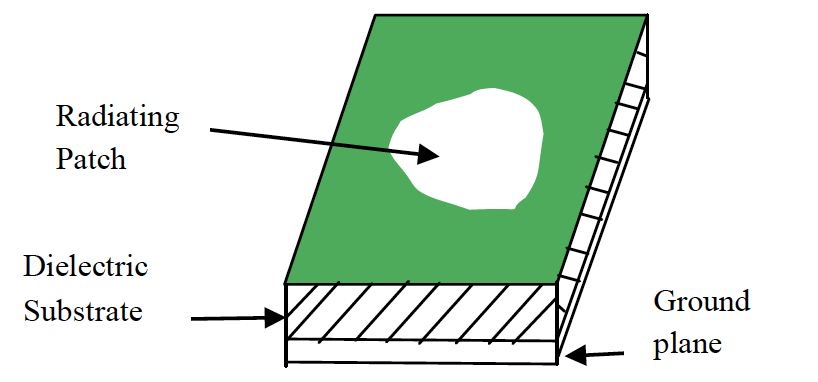
\includegraphics[width=\textwidth/2]{../images/patchantenna.png}
  \caption{General design of a microstrip antenna.}
  \label{fig:basicpatchantenna}
\end{figure}

The microstrip antenna requires besides the groundplane, dielectric substrate and the radiation patch also a feed line. Several feeding techniques exist of which the most popular are: coaxial probe feeding, microstrip line and aperture coupling. %and Microstrip Patch Antenna
%(todo: more refs? gebruik nummer twee van J13 (p2))

A first feeding method is with the usage of a coaxial cable where the outer conductor is attached to the ground plane and the inner conductor to the radiations patch. Modelling is however difficult, especially for thick substrates as will be used in this master dissertation.
A second option is the usage of a microstrip line. This type of feeding is much easier to model since the microstrip line can be seen as en extension of the radiating patch.
A disadvantage is the increased \gls{spuriousradiation} which limits bandwidth.
A third is proximity coupling which has the largest bandwidth and low \gls{spuriousradiation}. It consists however of two dielectric substrates causing the overall thickness
of the antenna to increase as well as its fabrication difficulty \cite{J13_singh2011micro}.
%(todo: tekst te weinig, bespreek ook apperture coupled attenna (zelfde paper als de rest))

The increasing usage of the microstrip patch antennae can be explained by it's easy fabrication and lightweightness and therefore knows a widespread application in the millitary, global possitioning systems, telemedicine, WiMAX applications and so on.
The authors of \cite{J13_microstripadvantages} also state that some of the disadvantages like lower gain and power handling can be solved with the usage of an array configuration.

The radiating patch is usually made of a thin layer of either gold or copper \cite{J14_antennadesign,J15_antennadesign}
and can have any form. However, shapes other than circles or rectangles would require large numerical computation \cite{J14_antennadesign}.
Thus, a simple rectangular shape will be used.
Further, also the dielectric constant of the substrate is important. It typically varies between 2.2 and 12.
Finding a good dielectric depends on how the antenna will used. A lower
dielectric constant with a thick substrate will result in better performance, better efficiency and larger bandwidths  \cite{J15_antennadesign}.
On the other hand, a larger dielectric constant reduces de dimensions of the antenna \cite{J14_antennadesign}
which is also useful when attaching the 
antenna to a limited surface. Glass as a dielectric substrate with a constant of 4.4 will be used.